\documentclass[12pt]{article}

% packages
\usepackage{setspace}
\usepackage{tikz}
\usepackage{array}
\usepackage[margin=0.75in]{geometry}
\usepackage{amsmath,bm}
\usepackage{amssymb}
\usepackage{bbold}
\usepackage{physics}
\usepackage{xcolor}
\usepackage{indentfirst}
\usepackage{enumerate}
\usepackage{mathtools}
\usepackage{cancel}

\doublespacing
\allowdisplaybreaks

\title{Notes on SSE for TFIM + $Z$-Field (LTFIM) at Finite Temperature}
\author{Isaac De Vlugt}
\date{\today}
\begin{document}

\maketitle

\section{Introduction}

This is motivated by our need to make an SSE QMC for the Rydberg hamiltonian.
\begin{align}
    H = & -h \sum_{i = 1}^N \sigma^x_i - \Omega \sum_{i=1}^n n_i - \sum_{\expval{i,j}} V_{ij} n_i n_j
\end{align}
Here, $n_i$ is simply an occupation number (i.e. either 0 or 1). We can therefore trivially map this to spin-$\frac{1}{2}$ with $n_i = \frac{1}{2}\left(\sigma_i^z + \mathbb{1} \right)$. The hamiltonian then becomes the following.
\begin{subequations}
    \begin{align}
        H = & - h \sum_{i = 1}^N \sigma^x_i - \frac{\Omega}{2} \sum_{i=1}^N \left(\sigma_i^z + \mathbb{1}\right) - \sum_{\expval{i,j}} V_{ij} \left(\sigma_i^z + \mathbb{1}\right) \left(\sigma_j^z + \mathbb{1}\right) \\
        =   & - h \sum_{i = 1}^N \sigma^x_i - \frac{\Omega}{2} \sum_{i=1}^N \left(\sigma_i^z + \mathbb{1}\right) - \sum_{\expval{i,j}} V_{ij} \left(\sigma_i^z \sigma_j^z + \sigma_i^z + \sigma_j^z + \mathbb{1}\right)
    \end{align}
\end{subequations}

\section{Longitudinal Field TFIM (LTFIM)}

The Rydberg Hamiltonian is extremely similar to a LTFIM (general $J_{ij}$ for all pairs, assuming $J_{ij} > 0 \quad \forall \quad i,j$ as in the Rydberg case since $V_{ij} = \frac{C}{R_{ij}^6}$).
\begin{align} \label{eq:LTFIM_hamiltonian}
    H = & - h \sum_{i = 1}^N \sigma^x_i - \Omega \sum_{i=1}^N \sigma_i^z + \sum_{\expval{i,j}} J_{ij} \sigma_i^z \sigma_j^z \qquad \mathrm{LTFIM}
\end{align}
Thus, if an efficient SSE formalism exists for such a Hamiltonian, then it is foreseeable that one may exist for the Rydberg Hamiltonian. So, let's work with the LTFIM as a toy model for the Rydberg Hamiltonian.

\subsection{Decomposition of Hamiltonian} \label{sec:H_decomp}

We first must decompose the Hamiltonian in Eq.~\eqref{eq:LTFIM_hamiltonian} in the form
\begin{align}
    H = - \sum_{t,a} H_{t,a},
\end{align}
where $t$ denotes the the type of $H_{t,a}$ (usually off-diagonal versus diagonal operators) and $a$ denotes the lattice unit over which the operator acts (i.e. sites, bonds, plaquettes, etc).
Inspiration can be taken from Sandvik's directed loops paper, wherein the XXZ model is explored in great detail. 
\begin{subequations} \label{eq:decomposition}
    \begin{align}
        H_{0,0} =& \mathbb{1} \\
        H_{-1,a} =& h \sigma_i^x \\
        H_{1,a} =& h \\
        H_{1,b} =& J \sigma_i^z \sigma_j^z + \Omega_b (\sigma_i^z + \sigma_j^z) + C
    \end{align}
\end{subequations}
Here, 
\begin{equation}
    \Omega_b = \frac{N\Omega}{2N_b}
\end{equation}
is the modified logitudinal field strength to account for over counting when the sum over sites is put into the sum over bonds.
This general expression accounts for PBCs, OBCs, and any lattice dimension.
$C = \max(J, 2 \Omega_b - J) + \varepsilon$ is a constant to aleviate sign problems with $H_{1,b}$, and $\varepsilon$ is a small non-negative constant to aid with numerics. 
In all, we have added a constant shift to Eq.~\eqref{eq:LTFIM_hamiltonian} of $N_b C + Nh$ that must be accounted for when calculating the energy. 

The non-zero matrix elements of all parts of the Hamiltonian (Eq.~\eqref{eq:decomposition}) are
\begin{subequations} \label{eq:mat_elems}
    \begin{align}
        \matrixel{\uparrow}{H_{-1,a}}{\downarrow} = \matrixel{\downarrow}{H_{-1,a}}{\uparrow} =& h \\
        \matrixel{\uparrow}{H_{1,a}}{\uparrow} = \matrixel{\downarrow}{H_{1,a}}{\downarrow} =& h \\
        W_1 \equiv \matrixel{\uparrow \uparrow}{H_{1,b}}{\uparrow \uparrow} =& J + 2\Omega_b + C \\
        W_2 \equiv \matrixel{\downarrow \downarrow}{H_{1,b}}{\downarrow \downarrow} =& J - 2\Omega_b + C \\
        W_3 \equiv \matrixel{\downarrow \uparrow}{H_{1,b}}{\downarrow \uparrow} = \matrixel{\uparrow \downarrow}{H_{1,b}}{\uparrow \downarrow} =& -J + C
    \end{align}
\end{subequations}

\subsection{Diagonal Updates}

We may have to toy around with the following procedures, but the general flow of things should be the same no matter what.
Given that the matrix elements of the diagonal operators are not the same, we must keep track of the propagated spin state $\ket{\alpha_p}$ at every time-slice.
For proposal modifications to the simulation cell, I will use primes.
Traverse the operator list and,
\begin{enumerate}
    \item if $H_{1,a}$ is encountered remove it ($n \rightarrow n - 1$) with probability
          \begin{align*}
              P_{[1,a]_p \rightarrow [0,0]_p} =& \mathrm{min}\left( \frac{1}{N}\frac{W^\prime(\alpha(p), S_M)}{W(\alpha(p), S_M)}, 1 \right) \\
              =& \mathrm{min}\left( \frac{\beta^{n-1}(M-(n-1))!}{N \times M!} \prod_{i=1}^{M} \matrixel{\alpha_{i-1}}{H_{t_i,a_i}}{\alpha_i}^\prime \times \frac{M!}{\beta^n(M-n)!} \left[\prod_{i=1}^{M} \matrixel{\alpha_{i-1}}{H_{t_i,a_i}}{\alpha_i}\right]^{-1}, 1 \right) \\
              =& \mathrm{min}\left(\frac{M-n+1}{\beta Nh },1\right).
          \end{align*}
    The factor of $N$ in the denominator is from the fact that where the operator $H_{1,a}$ is when we remove it does not matter. {\color{red} Is this right? Or do we not need the factor of $N$ anymore?} 
    \item if $H_{1,b}$ is encountered remove it ($n \rightarrow n - 1$) with probability
          \begin{align*}
              P_{[1,b]_p \rightarrow [0,0]_p} =& \mathrm{min}\left( \frac{W^\prime(\alpha(p), S_M)}{W(\alpha(p), S_M)}, 1 \right) \\
              =& \mathrm{min}\left( \frac{\beta^{n-1}(M-(n-1))!}{M!} \prod_{i=1}^{M} \matrixel{\alpha_{i-1}}{H_{t_i,a_i}}{\alpha_i}^\prime \times \frac{M!}{\beta^n(M-n)!} \left[\prod_{i=1}^{M} \matrixel{\alpha_{i-1}}{H_{t_i,a_i}}{\alpha_i}\right]^{-1}, 1 \right) \\
              =& \begin{cases}
                \mathrm{min}\left(\frac{M-n+1}{ \beta N_{\uparrow\uparrow} (J + 2\Omega_b + C) },1\right); & W_1 \\
                \mathrm{min}\left(\frac{M-n+1}{ \beta N_{\downarrow\downarrow} (J - 2\Omega_b + C) },1\right); & W_2 \\
                \mathrm{min}\left(\frac{M-n+1}{ \beta N_{\uparrow\downarrow / \downarrow\uparrow} (C - J) },1\right); & W_3 \\
              \end{cases}
          \end{align*}
    where $N_{\uparrow\uparrow}$, $N_{\downarrow\downarrow}$, and $N_{\uparrow\downarrow / \downarrow\uparrow}$ are the number of bonds at the current time slice with the corresponding spin configuration.
    Note that $N_{\uparrow\uparrow} + N_{\downarrow\downarrow} + N_{\uparrow\downarrow / \downarrow\uparrow} = N_b$.
    \item if the unity operator $H_{0,0}$ is encountered, insert a diagonal operator with the following procedure.
    First note that $W(A \text{ or } B \text{ or } C) = W(A) + W(B) + W(C)$. 
          \begin{itemize}
              \item Decide whether or not to insert a diagonal operator with the probability ($n \rightarrow n + 1$)
                    \begin{align*}
                        P_{H_{[1,a]_p} \text{ or } H_{[1,b]_p}} =& \mathrm{min}\left( \frac{W(H_{[1,a]_p} \text{ or } H_{[1,b]_{p,\uparrow\uparrow}} \text{ or } H_{[1,b]_{p,\downarrow\downarrow}} \text{ or } H_{[1,b]_{p,\uparrow\downarrow / \downarrow\uparrow}}) }{W(H_{[0,0]_p})} , 1 \right) \\
                        P_{H_{[1,a]_p} \text{ or } H_{[1,b]_p}} =& \mathrm{min}\left( \frac{W(H_{[1,a]_p}) + W(H_{[1,b]_{p,\uparrow\uparrow}}) + W(H_{[1,b]_{p,\downarrow\downarrow}}) + W(H_{[1,b]_{p,\uparrow\downarrow / \downarrow\uparrow}}) }{W(H_{[0,0]_p})} , 1 \right) \\
                        P_{H_{[1,a]_p} \text{ or } H_{[1,b]_p}} =& \mathrm{min}\left( \frac{\beta[Nh + N_{\uparrow\uparrow}(J + 2\Omega_b + C) + N_{\downarrow\downarrow}(J - 2\Omega_b + C) + N_{\uparrow\downarrow / \downarrow\uparrow}(C - J)]}{M - n} , 1 \right)
                    \end{align*}
                    \begin{align}
                        P_{H_{[1,a]_p} \text{ or } H_{[1,b]_p}} =& \mathrm{min}\left( \frac{\beta[Nh + N_{\uparrow\uparrow}(J + 2\Omega_b) + N_{\downarrow\downarrow}(J - 2\Omega_b) - N_{\uparrow\downarrow / \downarrow\uparrow}J + N_bC]}{M - n} , 1 \right)
                    \end{align}
              \item If it was decided to insert a diagonal operator, choose the operator to insert with probabilities
                    \begin{align}
                        P_{H_{[1,b]_p},\uparrow\uparrow} = & \frac{N_{\uparrow\uparrow}(J + 2\Omega_b + C)}{Nh + 4N_bC}, \\
                        P_{H_{[1,b]_p},\downarrow\downarrow} = & \frac{N_{\downarrow\downarrow}(J - 2\Omega_b + C)}{Nh + 4N_bC}, \\
                        P_{H_{[1,b]_p},\uparrow\downarrow / \downarrow\uparrow} = & \frac{N_{\uparrow\downarrow / \downarrow\uparrow}(C - J)}{Nh + 4N_bC}, \\
                        P_{H_{[1,a]_p}} =& \frac{Nh}{Nh + 4N_bC}
                    \end{align}
                \item If it was decided to insert $H_{1,a}$, then choose a random site (probability $1 / N$) to put the operator. Note that it can be put at any site regardless of spin! \\

                If it was decided to insert $H_{1,b}$, choose a bond according to the weights of each matrix element (i.e. find the up-up, down-down, and anti-parallel bonds and choose a bond according to heatbath probabilities associated with $W_1, W_2$ and $W_3$).
          \end{itemize}
\end{enumerate}

\subsection{Loop Updates}

In the spirit of the TFIM SSE formalism, we may still terminate on site operators $H_{1,a}$ and $H_{-1,a}$. 
However, loop formation is not deterministic since the matrix elements of $H_{1,b}$ are not all the same.
Therefore, we must devise a non-deterministic loop formation algorithm wherein detailed balance (DB) is satisfied.

\subsection{Detailed balance}

Recall the DB requirement given a configuration $s$ and $s^\prime$.
\begin{align} \label{eq:detailed_balance}
    P(s \rightarrow s^\prime)W(s) = P(s^\prime \rightarrow s)W(s^\prime)
\end{align}
It turns out that for detailed balance to be satisfied when loop segments reach a vertex associated with $H_{1,b}$, the following two equations must be satisfied.
\begin{subequations} \label{eq:db_requirements}
    \begin{align}
        W(s,\ell_1,\ell_2) =& W(s^\prime, \ell_2, \ell_1) \label{eq:db_1} \\
        \sum_x W(s,e,x) =& W_s \label{eq:db_2}
    \end{align}
\end{subequations}
\begin{itemize}
    \item $s$, $s^\prime$: vertex with it's four legs specified (legs being the spin states surrounding the operator $H_{1,b}$) 
    \item $e$: the leg that the loop segment enters
    \item $x$: the leg that the loop segment exits
    \item $\sum_x$: a sum over all exit paths (given a vertex $s$ and an entrace leg $e$)
    \item $W_s$: the matrix element of a single vertex with its four legs encoded as $s$
    \item $W(s,e,x) = W_s P(s,e \rightarrow s^\prime, x)$
\end{itemize}
Eq.~\eqref{eq:db_requirements} define the direted loop equations that must be satisfied for DB. 

\subsection{Directed loop equations}

To obtain directed loop equations and devise ways to satisfy them, we need to first look at possible loop segments through vertices corresponding to matrix elements of $H_{1,b}$.
Following Sandvik's directed loops paper, any ``switch'' loop segment (i.e. a segment whose exit leg is not the same lattice site as the entrance leg) will not be allowed since flipping the entrance and exit legs will yield off-diagonal matrix element of $H_{1,b}$, which is non-existant ($H_{1,b}$ is a diagonal operator).
Therefore, the only two loop segments that are allowed are ``continue straight'' or ``bounce''. See Fig.~\ref{fig:continue_bounce}. 

\begin{figure}
    \centering
    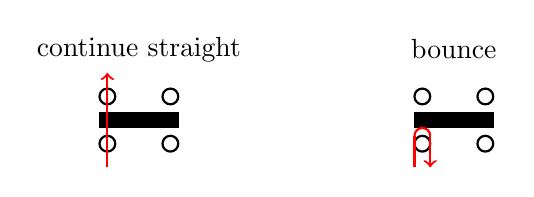
\begin{tikzpicture}

        % new

        \filldraw[black] (0.5, 1) node[anchor=center] {continue straight};

        \draw[thick] (0.1,0.4) circle (0.1); % UL
        \draw[thick] (0.9,0.4) circle (0.1); % UR
        \draw[thick] (0.1,-0.2) circle (0.1); % LL
        \draw[thick] (0.9,-0.2) circle (0.1); % LR

        \draw[black, fill=black] (0,0) rectangle (1,0.2);

        \draw[red, thick, ->] (0.1,-0.5) -- (0.1,0.7);

        % new

        \filldraw[black] (4.5, 1) node[anchor=center] {bounce};

        \draw[thick] (4.1,0.4) circle (0.1); % UL
        \draw[thick] (4.9,0.4) circle (0.1); % UR
        \draw[thick] (4.1,-0.2) circle (0.1); % LL
        \draw[thick] (4.9,-0.2) circle (0.1); % LR

        \draw[black, fill=black] (4,0) rectangle (5,0.2);

        \draw[red, thick] (4,-0.5) -- (4,-0.1);
        \draw[red, thick] (4,-0.1) arc (180:0:0.1);
        \draw[red, thick, ->] (4.2,-0.1) -- (4.2,-0.5);

    \end{tikzpicture}    
\caption{...} \label{fig:continue_bounce}
\end{figure}

For loop segments to satisfy DB, we must relate vertices in which the two spins that are connected by the segment are flipped and the direction of the segment if reversed. 
An example is in Fig.~\ref{fig:related_vertices}.

\begin{figure} [!h]
    \centering
    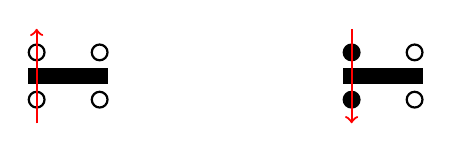
\begin{tikzpicture}

        % new

        \draw[thick] (0.1,0.4) circle (0.1); % UL
        \draw[thick] (0.9,0.4) circle (0.1); % UR
        \draw[thick] (0.1,-0.2) circle (0.1); % LL
        \draw[thick] (0.9,-0.2) circle (0.1); % LR

        \draw[black, fill=black] (0,0) rectangle (1,0.2);

        \draw[red, thick, ->] (0.1,-0.5) -- (0.1,0.7);

        % new

        \draw[thick, fill=black] (4.1,0.4) circle (0.1); % UL
        \draw[thick] (4.9,0.4) circle (0.1); % UR
        \draw[thick, fill=black] (4.1,-0.2) circle (0.1); % LL
        \draw[thick] (4.9,-0.2) circle (0.1); % LR

        \draw[black, fill=black] (4,0) rectangle (5,0.2);

        \draw[red, thick, ->] (4.1,0.7) -- (4.1,-0.5);

    \end{tikzpicture}    
\caption{...} \label{fig:related_vertices}
\end{figure}
Mathematically, these graphs represent the equivalence relation Eq.~\ref{eq:db_1}.
Note that the bounce loop segments map to themselves under this transformation (flipping spins, reversing loop segment direction).
Furthermore, Eq.~\ref{eq:db_2} relates vertices with different exit legs having the same spin configuration and entrance leg.
Graphically, the sum of the graphs in Fig.~\ref{fig:continue_bounce} must be equal to $W_3$ (here, we use filled/unfilled dots to represent spin-up/down).

Now, let's look at the directed loop equations. 
It's at this point that where we refer to the directed loops paper, specifically Fig. 8.
This figure outlines that all possible vertex configurations can be divided into 8 subsets that don't transform into each other as dictated by Eq.~\ref{eq:db_1}.
It's a little different/simpler in our case (i.e. XXZ model versus LTFIM), since we cannot have any "switch" loop segments.
The other 4 subsets of related vertices are simply those in Fig.~\ref{fig:vertex_subsets} but with the spins flipped.
Each configuration in a given quadrant maps to another configuration in the same quadrant (i.e. similar to Fig.~\ref{fig:related_vertices}). 
Again, bounce operations map to themselves.

\begin{figure}
    \centering
    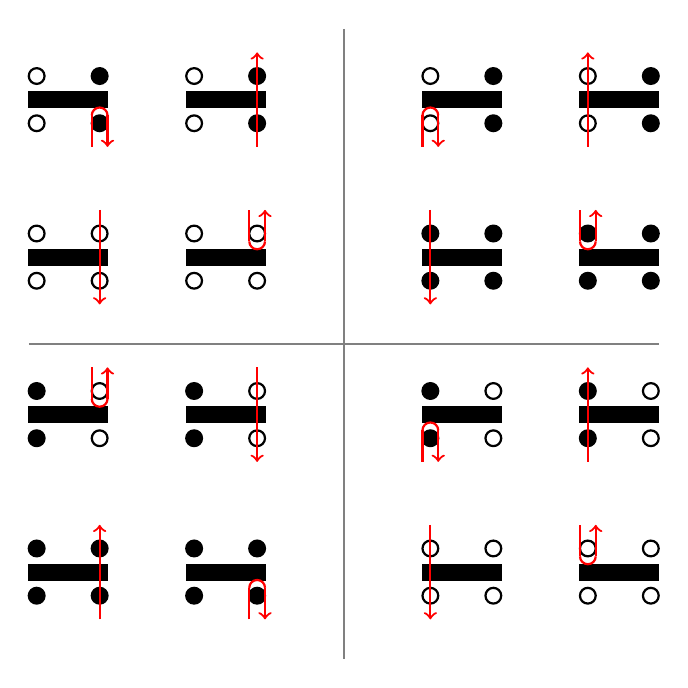
\begin{tikzpicture}

        \draw[gray, thick] (0,-3) -- (8,-3);
        \draw[gray, thick] (4, 1) -- (4, -7);

        % new 1,1

        \draw[thick] (0.1,0.4) circle (0.1); % UL
        \draw[fill=black,thick] (0.9,0.4) circle (0.1); % UR
        \draw[thick] (0.1,-0.2) circle (0.1); % LL
        \draw[fill=black,thick] (0.9,-0.2) circle (0.1); % LR

        \draw[black, fill=black] (0,0) rectangle (1,0.2);

        \draw[red, thick] (0.8,-0.5) -- (0.8,-0.1);
        \draw[red, thick] (0.8,-0.1) arc (180:0:0.1);
        \draw[red, thick, ->] (1,-0.1) -- (1,-0.5);

        % new 1,2

        \draw[thick] (2.1,0.4) circle (0.1); % UL
        \draw[fill=black,thick] (2.9,0.4) circle (0.1); % UR
        \draw[thick] (2.1,-0.2) circle (0.1); % LL
        \draw[fill=black,thick] (2.9,-0.2) circle (0.1); % LR

        \draw[black, fill=black] (2,0) rectangle (3,0.2);

        \draw[red, thick, ->] (2.9,-0.5) -- (2.9,0.7);

        % new 1,3

        \draw[thick] (0.1,-1.6) circle (0.1); % UL
        \draw[thick] (0.9,-1.6) circle (0.1); % UR
        \draw[thick] (0.1,-2.2) circle (0.1); % LL
        \draw[thick] (0.9,-2.2) circle (0.1); % LR

        \draw[black, fill=black] (0,-2) rectangle (1,-1.8);

        \draw[red, thick, ->] (0.9,-1.3) -- (0.9,-2.5);

        % new 1,4

        \draw[thick] (2.1,-1.6) circle (0.1); % UL
        \draw[thick] (2.9,-1.6) circle (0.1); % UR
        \draw[thick] (2.1,-2.2) circle (0.1); % LL
        \draw[thick] (2.9,-2.2) circle (0.1); % LR

        \draw[black, fill=black] (2,-2) rectangle (3,-1.8);

        \draw[red, thick] (2.8,-1.7) -- (2.8,-1.3);
        \draw[red, thick] (2.8,-1.7) arc (180:360:0.1);
        \draw[red, thick, ->] (3,-1.7) -- (3,-1.3);

        % new 2,1

        \draw[thick] (5.1,0.4) circle (0.1); % UL
        \draw[fill=black,thick] (5.9,0.4) circle (0.1); % UR
        \draw[thick] (5.1,-0.2) circle (0.1); % LL
        \draw[fill=black,thick] (5.9,-0.2) circle (0.1); % LR

        \draw[black, fill=black] (5,0) rectangle (6,0.2);

        \draw[red, thick] (5,-0.5) -- (5,-0.1);
        \draw[red, thick] (5,-0.1) arc (180:0:0.1);
        \draw[red, thick, ->] (5.2,-0.1) -- (5.2,-0.5);

        % new 2,2

        \draw[thick] (7.1,0.4) circle (0.1); % UL
        \draw[fill=black,thick] (7.9,0.4) circle (0.1); % UR
        \draw[thick] (7.1,-0.2) circle (0.1); % LL
        \draw[fill=black,thick] (7.9,-0.2) circle (0.1); % LR

        \draw[black, fill=black] (7,0) rectangle (8,0.2);

        \draw[red, thick, ->] (7.1,-0.5) -- (7.1,0.7);

        % new 2,3

        \draw[fill=black,thick] (5.1,-1.6) circle (0.1); % UL
        \draw[fill=black,thick] (5.9,-1.6) circle (0.1); % UR
        \draw[fill=black,thick] (5.1,-2.2) circle (0.1); % LL
        \draw[fill=black,thick] (5.9,-2.2) circle (0.1); % LR

        \draw[black, fill=black] (5,-2) rectangle (6,-1.8);

        \draw[red, thick, ->] (5.1,-1.3) -- (5.1,-2.5);

        % new 2,4

        \draw[fill=black,thick] (7.1,-1.6) circle (0.1); % UL
        \draw[fill=black,thick] (7.9,-1.6) circle (0.1); % UR
        \draw[fill=black,thick] (7.1,-2.2) circle (0.1); % LL
        \draw[fill=black,thick] (7.9,-2.2) circle (0.1); % LR

        \draw[black, fill=black] (7,-2) rectangle (8,-1.8);

        \draw[red, thick] (7,-1.7) -- (7,-1.3);
        \draw[red, thick] (7,-1.7) arc (180:360:0.1);
        \draw[red, thick, ->] (7.2,-1.7) -- (7.2,-1.3);

        % new 3,1

        \draw[fill=black,thick] (0.1,-3.6) circle (0.1); % UL
        \draw[thick] (0.9,-3.6) circle (0.1); % UR
        \draw[fill=black,thick] (0.1,-4.2) circle (0.1); % LL
        \draw[thick] (0.9,-4.2) circle (0.1); % LR

        \draw[black, fill=black] (0,-4) rectangle (1,-3.8);

        \draw[red, thick] (0.8,-3.7) -- (0.8,-3.3);
        \draw[red, thick] (0.8,-3.7) arc (180:360:0.1);
        \draw[red, thick, ->] (1,-3.7) -- (1,-3.3);

        % new 3,2

        \draw[fill=black,thick] (2.1,-3.6) circle (0.1); % UL
        \draw[thick] (2.9,-3.6) circle (0.1); % UR
        \draw[fill=black,thick] (2.1,-4.2) circle (0.1); % LL
        \draw[thick] (2.9,-4.2) circle (0.1); % LR

        \draw[black, fill=black] (2,-4) rectangle (3,-3.8);

        \draw[red, thick, ->] (2.9,-3.3) -- (2.9,-4.5);

        % new 3,3

        \draw[fill=black,thick] (0.1,-5.6) circle (0.1); % UL
        \draw[fill=black,thick] (0.9,-5.6) circle (0.1); % UR
        \draw[fill=black,thick] (0.1,-6.2) circle (0.1); % LL
        \draw[fill=black,thick] (0.9,-6.2) circle (0.1); % LR

        \draw[black, fill=black] (0,-6) rectangle (1,-5.8);

        \draw[red, thick, ->] (0.9,-6.5) -- (0.9,-5.3);

        % new 3,4

        \draw[fill=black,thick] (2.1,-5.6) circle (0.1); % UL
        \draw[fill=black,thick] (2.9,-5.6) circle (0.1); % UR
        \draw[fill=black,thick] (2.1,-6.2) circle (0.1); % LL
        \draw[fill=black,thick] (2.9,-6.2) circle (0.1); % LR

        \draw[black, fill=black] (2,-6) rectangle (3,-5.8);

        \draw[red, thick] (2.8,-6.5) -- (2.8,-6.1);
        \draw[red, thick] (2.8,-6.1) arc (180:0:0.1);
        \draw[red, thick, ->] (3,-6.1) -- (3,-6.5);

        % new 4,1

        \draw[fill=black,thick] (5.1,-3.6) circle (0.1); % UL
        \draw[thick] (5.9,-3.6) circle (0.1); % UR
        \draw[fill=black,thick] (5.1,-4.2) circle (0.1); % LL
        \draw[thick] (5.9,-4.2) circle (0.1); % LR

        \draw[black, fill=black] (5,-4) rectangle (6,-3.8);

        \draw[red, thick] (5,-4.5) -- (5,-4.1);
        \draw[red, thick] (5,-4.1) arc (180:0:0.1);
        \draw[red, thick, ->] (5.2,-4.1) -- (5.2,-4.5);

        % new 4,2

        \draw[fill=black,thick] (7.1,-3.6) circle (0.1); % UL
        \draw[thick] (7.9,-3.6) circle (0.1); % UR
        \draw[fill=black,thick] (7.1,-4.2) circle (0.1); % LL
        \draw[thick] (7.9,-4.2) circle (0.1); % LR

        \draw[black, fill=black] (7,-4) rectangle (8,-3.8);

        \draw[red, thick, ->] (7.1,-4.5) -- (7.1,-3.3);

        % new 4,3

        \draw[thick] (5.1,-5.6) circle (0.1); % UL
        \draw[thick] (5.9,-5.6) circle (0.1); % UR
        \draw[thick] (5.1,-6.2) circle (0.1); % LL
        \draw[thick] (5.9,-6.2) circle (0.1); % LR

        \draw[black, fill=black] (5,-6) rectangle (6,-5.8);

        \draw[red, thick, ->] (5.1,-5.3) -- (5.1,-6.5);

        % new 4,4

        \draw[thick] (7.1,-5.6) circle (0.1); % UL
        \draw[thick] (7.9,-5.6) circle (0.1); % UR
        \draw[thick] (7.1,-6.2) circle (0.1); % LL
        \draw[thick] (7.9,-6.2) circle (0.1); % LR

        \draw[black, fill=black] (7,-6) rectangle (8,-5.8);

        \draw[red, thick] (7,-5.7) -- (7,-5.3);
        \draw[red, thick] (7,-5.7) arc (180:360:0.1);
        \draw[red, thick, ->] (7.2,-5.7) -- (7.2,-5.3);

    \end{tikzpicture}    
\caption{...} \label{fig:vertex_subsets}
\end{figure}

Now this is where I am a little shady on some of the details. 
In the directed loops paper, Sandvik notes that there are two symmetries we can take advantage of in order to reduce the number of directed loop equations that we need to solve.
\begin{enumerate}
    \item Permutation of two spins acted on by $H_{1,b}$ (i.e. interchanging spins while keeping the orientation of the loop segment)
    \item Imaginary-time symmetry (swap spins above and below the black-filled bar that represents $H_{1,b}$)
\end{enumerate}
In all, this simplifies our directed loop equations to just those associated to the upper-left and lower-left quadrants (i.e. all other quadrants can be mapped back to the upper-left quadrant or lower-left quadrant). 

The directed loop equations for the upper-left quadrant are
\begin{subequations} \label{eq:directed_loop_eq1}
    \begin{align}
        W_3 = -J + C =& W(3,4,4) + W(3,4,2) = b_1 + a, \\
        W_2 = J - 2\Omega_b + C =& W(2,2,4) + W(2,2,2) = a + b_2.
    \end{align}
\end{subequations}
Note that we used Eq.~\ref{eq:db_1} to equate $W(3,4,2) = W(2,2,4) = a$.

For the lower-left quadrant, 
\begin{subequations} \label{eq:directed_loop_eq2}
    \begin{align}
        W_3 = -J + C =& W(3,2,2) + W(3,2,4) = b_3 + d, \\
        W_1 = J + 2\Omega_b + C =& W(1,4,2) + W(1,4,4) = d + b_4.
    \end{align}
\end{subequations}
Note that we used Eq.~\ref{eq:db_1} to equate $W(3,2,4) = W(1,4,2) = d$.
The variables $b_i$ denote bounce weights.

\subsubsection{Heat-bath solutions to directed loop equations}

If we reach the operator $H_{1,b}$ at a given leg, the probability of choosing an exit is given by the weight of the vertex with the spins connected by the loop segment being flipped. 
This is a standard heat-bath update scheme that satisfies detailed balance (proof in directed loops paper).
So, let's verify that these are indeed solutions to our directed loop equations.
I.e., it should be that
\begin{align*}
    \frac{b_1}{W_3} =& \frac{W_3^2}{W_3 + W_2} \\
    \frac{b_2}{W_2} =& \frac{W_2^2}{W_3 + W_2} \\
    \frac{a}{W_3} =& \frac{W_3 W_2}{W_3 + W_2},
\end{align*}
and
\begin{align*}
    \frac{b_3}{W_3} =& \frac{W_3^2}{W_1 + W_3} \\
    \frac{b_4}{W_1} =& \frac{W_1^2}{W_1 + W_3} \\
    \frac{d}{W_3} =& \frac{W_3 W_1}{W_1 + W_3},
\end{align*}
You can check that indeed, these are solutions.

\subsubsection{General solutions to directed loop equations}

While the heat-bath probabilties should work, it is not preferred that the bounce probabilities are non-zero since bouncing in effect does nothing to update the simulation cell.
Let's analyze how $b_i$ can be minimized whilst Eqs.~\ref{eq:directed_loop_eq1} and \ref{eq:directed_loop_eq2} are satisfied and $b_i, a, d \geq 0$ (no sign problems).
Let's solve for the $b_i$'s,

\begin{subequations}
    \begin{align}
        b_1 =& -a - J + C, \\
        b_2 =& -a + J - 2\Omega_b + C,
    \end{align}
\end{subequations}
and
\begin{subequations}
    \begin{align}
        b_3 =& -d - J + C, \\
        b_4 =& -d + J + 2\Omega_b + C.
    \end{align}
\end{subequations}

Clearly, the lines defining $b_{1,2}$ vs $a$ are parallel and will never intersect, similarily for the lines defining $b_{3,4}$ vs $d$.
So there doesn't exist a solution to Eqs.~\ref{eq:directed_loop_eq1} and \ref{eq:directed_loop_eq2} wherein $b_i = 0$ $\forall$ $b_i$.

\end{document}